\section{Part B: Regression Problem of the Graduate Admissions Predication dataset}
\label{part2}
The details of the dataset are given as follows:
\begin{quote}
This assignment uses the data from the Graduate Admissions Predication [2]. The dataset contains several parameters, like GRE score (out of 340), TOEFL score (out of 120), university Rating (out of 5), strengths of Statement of Purpose and Letter of Recommendation (out of 5), undergraduate GPA (out of 10), research experience (either 0 or 1), that are considered important during the application for Master Programs. The predicted parameter is the chance of getting an admit (ranging from 0 to 1). You can obtain the data from: https://www.kaggle.com/mohansacharya/graduate-admissions
\end{quote}

In this problem, the dataset is divided at a 70:30 ratio for training and testing.

The neural network is defined as in Listing \ref{ls:2_nn}, with the loss and weight regularisation functions defined in Listing \ref{ls:2_cost}.

\begin{lstlisting}[language=Python, caption= Feedforward neural network (layers controlled by layers parameter), label=ls:2_nn]
def ffn(x, feature_size, neuron_size, weight_decay_beta, layers=3, dropout=False):
    """Feedforward net with hidden layers
    """
    sum_regularization = 0
    with tf.name_scope('hidden'):
        weights = tf.Variable(tf.truncated_normal([feature_size, neuron_size], stddev=1.0 / np.sqrt(feature_size), dtype=tf.float32), name='weights')
        biases = tf.Variable(tf.zeros([neuron_size]), dtype=tf.float32, name='biases')
        h  = tf.nn.relu(tf.matmul(x, weights) + biases)
        if dropout:
            h = tf.nn.dropout(h, 0.8)
        sum_regularization += weight_decay_beta * tf.nn.l2_loss(weights)
    if layers > 3:
        for i in range(layers-3):
            with tf.name_scope('hidden{}'.format(i)):
                weights = tf.Variable(tf.truncated_normal([neuron_size, neuron_size], stddev=1.0 / np.sqrt(neuron_size), dtype=tf.float32), name='weights')
                biases = tf.Variable(tf.zeros([neuron_size]), dtype=tf.float32, name='biases')
                h  = tf.nn.relu(tf.matmul(h, weights) + biases)
                if dropout:
                    h = tf.nn.dropout(h, 0.8)
                sum_regularization += weight_decay_beta * tf.nn.l2_loss(weights)
    with tf.name_scope('linear'):
        weights = tf.Variable(tf.truncated_normal([neuron_size, 1], stddev=1.0 / np.sqrt(neuron_size), dtype=tf.float32), name='weights')
        biases  = tf.Variable(tf.zeros([1]), dtype=tf.float32, name='biases')
        u = tf.matmul(h, weights) + biases
        sum_regularization += weight_decay_beta * tf.nn.l2_loss(weights)


    return u, sum_regularization
\end{lstlisting}

\begin{lstlisting}[language=Python, caption= loss and weight regularisation functions, label=ls:2_cost]
def create_model(feature_size, neuron_size, weight_decay_beta, learning_rate, layers=3, dropout=False):
    # Create the model
    x = tf.placeholder(tf.float32, [None, feature_size])
    y_ = tf.placeholder(tf.float32, [None, 1])
    y, regularizer = ffn(x, feature_size, neuron_size, weight_decay_beta, layers=layers, dropout=dropout)

    #Create the gradient descent optimizer with the given learning rate.
    optimizer = tf.train.GradientDescentOptimizer(learning_rate)
    cost = tf.square(y_ - y)
    loss = tf.reduce_mean(cost + regularizer)
    train_op = optimizer.minimize(loss)
    return y, train_op, y_, x, loss
\end{lstlisting}

Mini-batch gradient descend is done through Listing \ref{ls:mini_batch}.

\begin{lstlisting}[language=Python, caption= Mini-batch, label=ls:mini_batch]
            for start, end in zip(range(0, len(train_x), batch_size), range(batch_size, len(train_x), batch_size)):
                train_op.run(feed_dict={x: train_x[start:end], y_: train_y[start:end]})
\end{lstlisting}

\subsection{Question 1}
\label{2q1}
\begin{quote}
1. Design a 3-layer feedforward neural network consists of an input layer, a hidden-layer of 10 neurons having ReLU activation functions, and a linear output layer. Use mini-batch gradient descent with a batch size = 8, L2
regularization at weight decay parameter = $10^{-3}$ and a learning rate = $10^{-3}$ to train the network.

a) Use the train dataset to train the model and plot both the train and test errors against epochs.

b) State the approximate number of epochs where the test error is minimum and use it to stop training.

c) Plot the predicted values and target values for any 50 test samples.
\end{quote}
\subsubsection{Part A}

\begin{figure}[H]
    \centering
    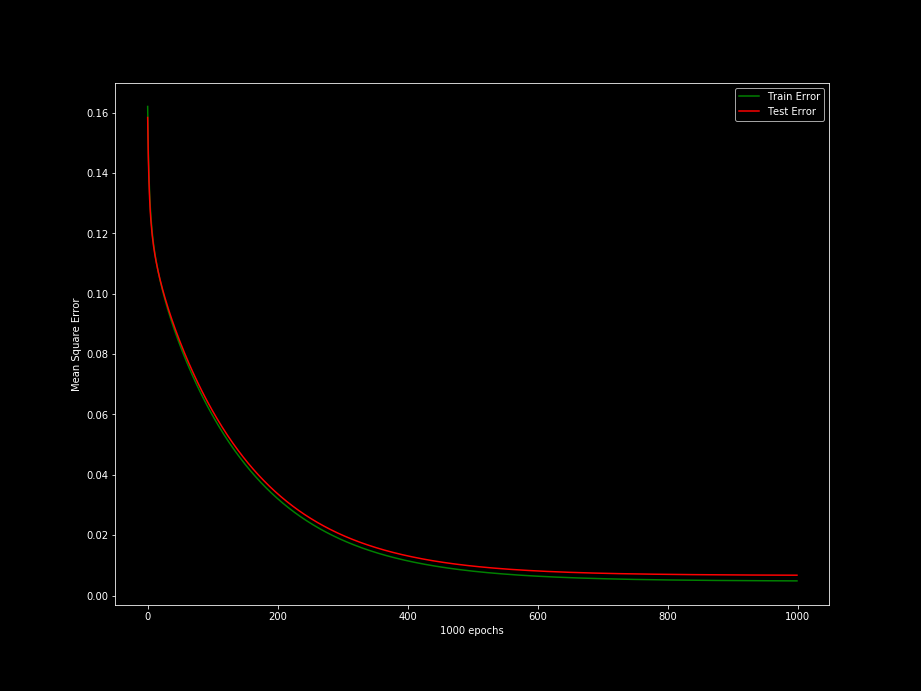
\includegraphics[width=0.8\linewidth]{assets/plots2/part2_Q1a.png}
    \caption{Plot of training and testing errors against epochs}
    \label{fig:2_1a}
\end{figure}

Figure \ref{fig:2_1a} shows the plot of training and testing errors against epochs for the 3-layer feedforward neural network as specified in the question.

\subsubsection{Part B}
Upon close inspection, it can be seen that the test error converges at around 900-1000 epochs. As such, we will use 1000 epochs as the point with minimum error.

\subsubsection{Part C}
\begin{figure}[H]
    \centering
    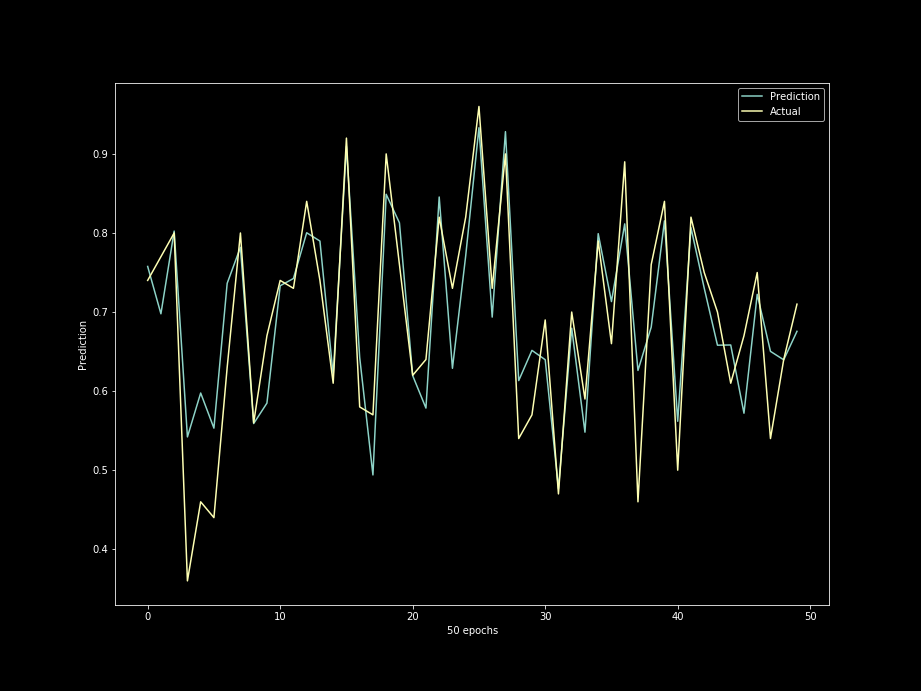
\includegraphics[width=0.8\linewidth]{assets/plots2/part2_Q1c.png}
    \caption{Plot of predicted values and target values against epochs for 50 test samples}
    \label{fig:2_1c}
\end{figure}

Figure \ref{fig:2_1c} shows the plot of predicted vs actual values. As can be seen from the plot, most predicted values are actually close to the actual values obtained. This is consistent with the low test error obtained in \ref{fig:2_1c}.

\subsection{Question 2}
\label{2q2}
\begin{quote}
2. Use the train data to compute (and plot) an 8X8 correlation matrix between the different feature scores and the corresponding chances of admit.

a) Which features are most correlated to each other? Is it justifiable?

b) What features have the highest correlations with the chances of admit?
\end{quote}
\subsubsection{Part A}

\begin{longtable}[c]{|c|c|c|c|c|c|c|c|c|}
\hline
\rowcolor[HTML]{85A4FF} 
 & \begin{tabular}[c]{@{}c@{}}GRE \\ Score\end{tabular} & \begin{tabular}[c]{@{}c@{}}TOEFL \\ Score\end{tabular} & \begin{tabular}[c]{@{}c@{}}University \\ Rating\end{tabular} & SOP & LOR & CGPA & Research & \begin{tabular}[c]{@{}c@{}}Chance \\ of Admit\end{tabular} \\ \hline
\endfirsthead
%
\endhead
%
\cellcolor[HTML]{C0C0C0}\begin{tabular}[c]{@{}c@{}}GRE \\ Score\end{tabular} & 1.0 & 0.836 & 0.669 & 0.613 & 0.558 & 0.833 & 0.580 & 0.803 \\ \hline
\cellcolor[HTML]{C0C0C0}\begin{tabular}[c]{@{}c@{}}TOEFL \\ Score\end{tabular} & 0.836 & 1.0 & 0.696 & 0.658 & 0.568 & 0.828 & 0.490 & 0.792 \\ \hline
\cellcolor[HTML]{C0C0C0}\begin{tabular}[c]{@{}c@{}}University \\ Rating\end{tabular} & 0.669 & 0.696 & 1.0 & 0.735 & 0.660 & 0.746 & 0.448 & 0.711 \\ \hline
\cellcolor[HTML]{C0C0C0}SOP & 0.613 & 0.658 & 0.735 & 1.0 & 0.730 & 0.718 & 0.444 & 0.676 \\ \hline
\cellcolor[HTML]{C0C0C0}LOR & 0.558 & 0.568 & 0.660 & 0.730 & 1.0 & 0.670 & 0.397 & 0.670 \\ \hline
\cellcolor[HTML]{C0C0C0}CGPA & 0.833 & 0.828 & 0.746 & 0.718 & 0.670 & 1.0 & 0.522 & 0.873 \\ \hline
\cellcolor[HTML]{C0C0C0}Research & 0.580 & 0.490 & 0.448 & 0.444 & 0.397 & 0.521 & 1.0 & 0.553 \\ \hline
\cellcolor[HTML]{C0C0C0}\begin{tabular}[c]{@{}c@{}}Chance \\ of Admit\end{tabular} & 0.803 & 0.792 & 0.711 & 0.676 & 0.670 & 0.873 & 0.553 & 1.0 \\ \hline
\caption{Correlation Matrix}
\label{tab:corr_matrix}\\
\end{longtable}

Table \ref{tab:corr_matrix} shows the 8x8 correlation matrix between the different feature scores and chance to admit. The features with the highest correlation with each other are the TOEFL Score and GRE Score. The relationship between both of them may be because the GRE Test is a critical thinking and reasoning test usually conducted in English, while TOEFL is a English proficiency test. Therefore if the student score higher in TOEFL, means they might more likely understand what the GRE Test contents are which could improve their scores.

\subsubsection{Part B}
CGPA is the feature that is the most correlated to Chance of Admit, while the GRE Score is the second most correlated to Chance of Admit.

\subsection{Question 3}
\label{2q3}
\begin{quote}
3. Recursive feature elimination (RFE) is a feature selection method that removes unnecessary features from the inputs. Start by removing one input feature that causes the minimum drop (or maximum improvement) in performance. Repeat the procedure recursively on the reduced input set until the optimal number of input features is reached. Remove the features one at a time. Compare the accuracy of the model with all input features, with models using 6 input features and 5 input features selected using RFE. Comment on the observations.
\end{quote}
\subsubsection{RFE iteration 1, with 6 features}
\begin{figure}[H]
    \begin{subfigure}{1\textwidth}
        \centering
        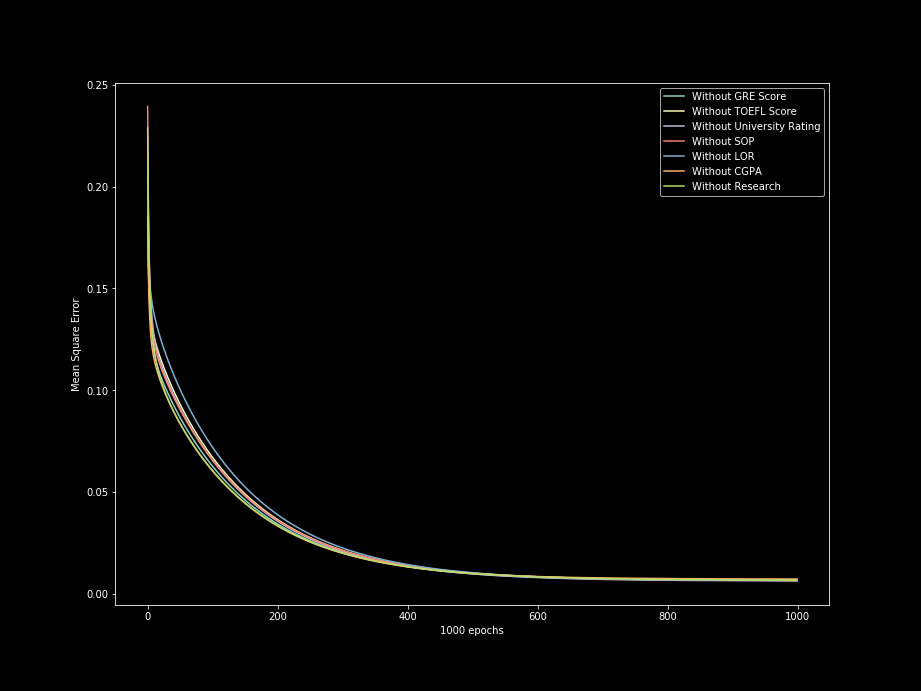
\includegraphics[width=0.8\linewidth]{assets/plots2/part3_2.png}
        \caption{Test error with RFE iteration 1}
        \label{fig:rfe1}
    \end{subfigure} 
\end{figure}
\begin{figure}[H]
    \ContinuedFloat
    \begin{subfigure}{1\textwidth}
        \centering
        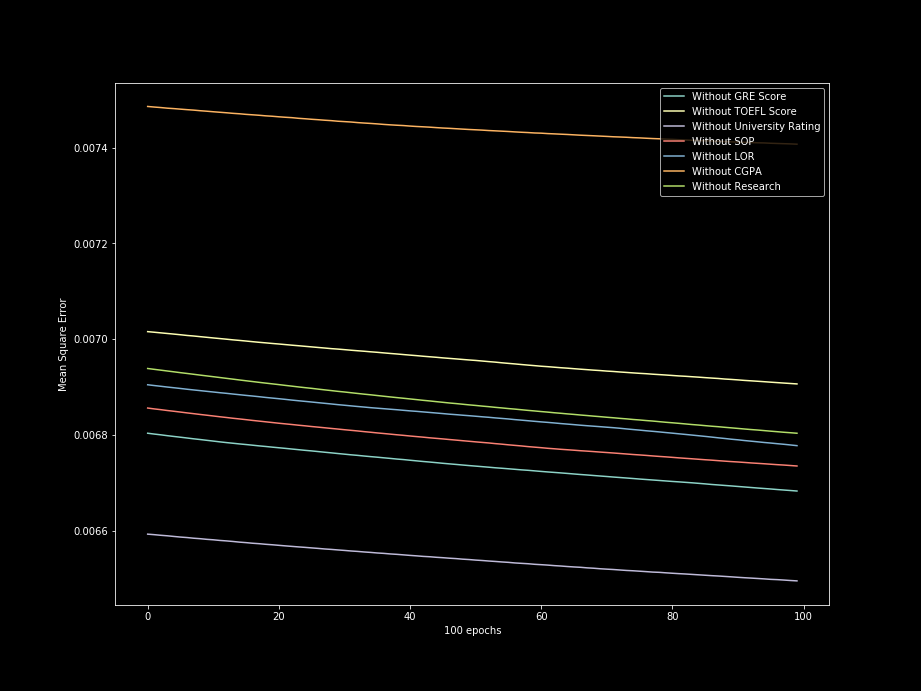
\includegraphics[width=0.8\linewidth]{assets/plots2/part3_3.png}
        \caption{Test error with RFE iteration 1 - last 100 epochs}
        \label{fig:rfe1_zoom}
    \end{subfigure}
\end{figure}

In the first iteration of RFE, it can be seen in Figure \ref{fig:rfe1_zoom} that University Ranking, followed by GRE, when removed, gives the least mean square error. This means that the removal of University Ranking will cause the least drop in performance for the model. Thus, we eliminate University Ranking in the first iteration of RFE.

\subsubsection{RFE iteration 2, with 5 features}
\begin{figure}[H]
    \begin{subfigure}{1\textwidth}
        \centering
        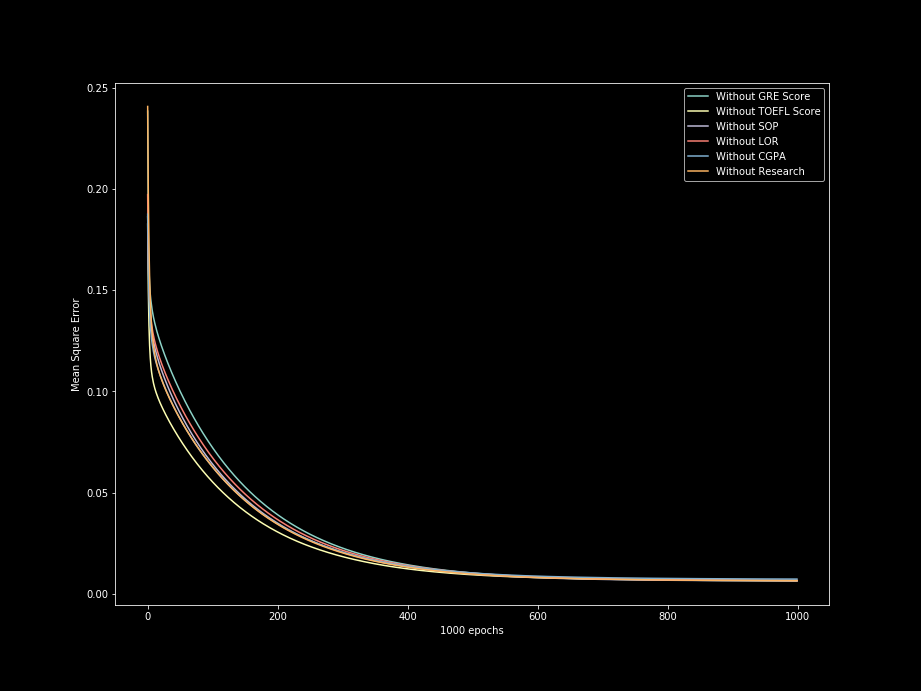
\includegraphics[width=0.8\linewidth]{assets/plots2/part3_5.png}
        \caption{Test error with RFE iteration 2}
        \label{fig:rfe2}
    \end{subfigure}
\end{figure}
\begin{figure}[H]
    \ContinuedFloat
    \begin{subfigure}{1\textwidth}
        \centering
        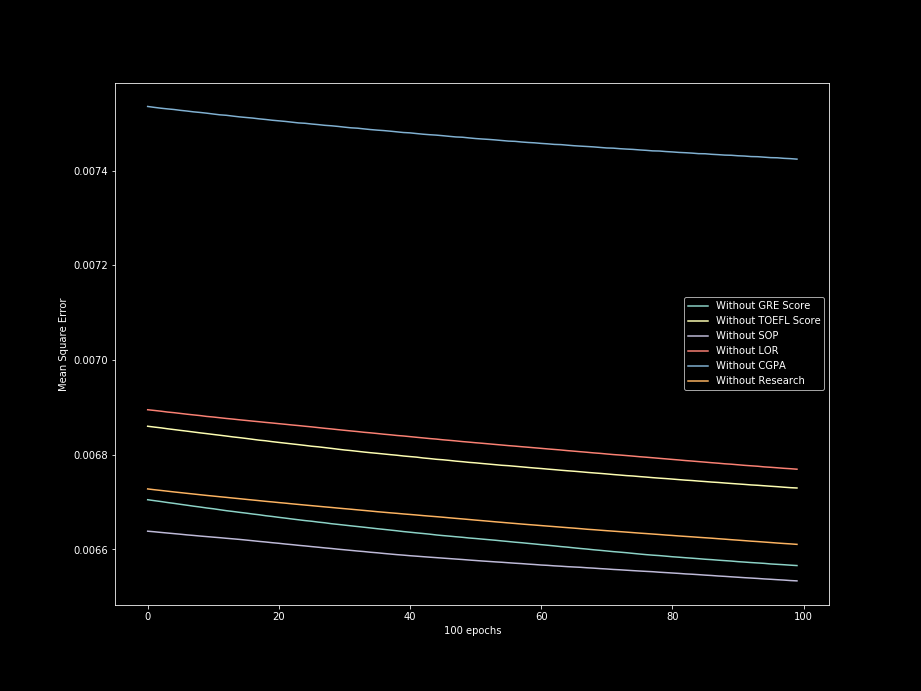
\includegraphics[width=0.8\linewidth]{assets/plots2/part3_6.png}
        \caption{Test error with RFE iteration 2 - last 100 epochs}
        \label{fig:rfe2_zoom}
    \end{subfigure}
\end{figure}

In the second iteration of RFE, it can be seen in Figure \ref{fig:rfe1_zoom} that the SOP when removed, gives the least mean square error. Similar to University Ranking, it means that the removal of SOP will cause the least drop in performance for the model. Therefore, we will remove this feature next in RFE.

\subsubsection{RFE comparisons}
\begin{figure}[H]
    \begin{subfigure}{1\textwidth}
        \centering
        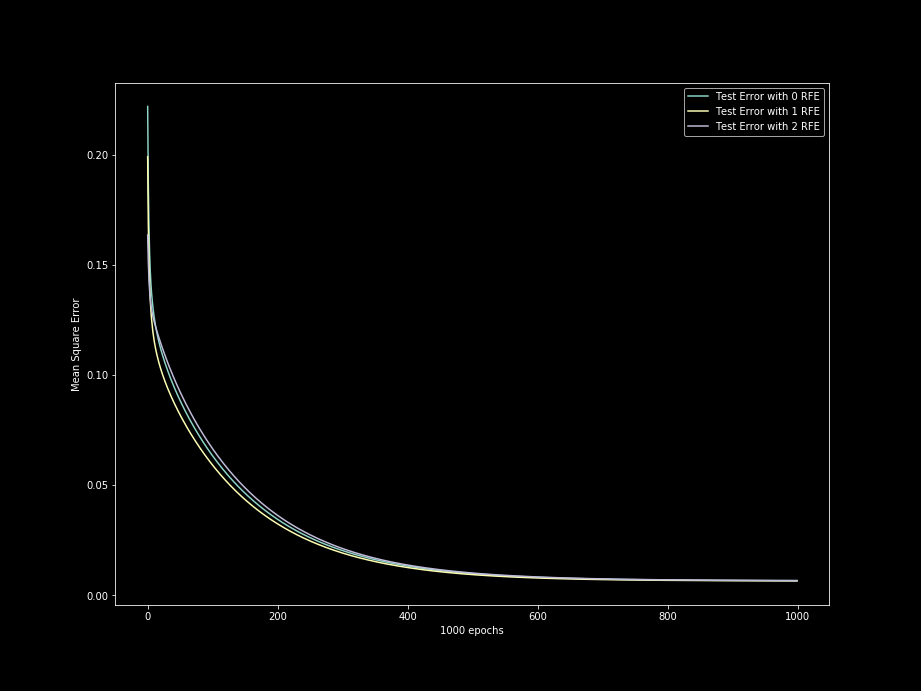
\includegraphics[width=0.8\linewidth]{assets/plots2/part3_7.png}
        \caption{Plot of accuracy predictions for different number of features removed by RFE}
        \label{fig:rfe3}
    \end{subfigure}
\end{figure}
\begin{figure}[H]
    \ContinuedFloat
    \begin{subfigure}{1\textwidth}
        \centering
        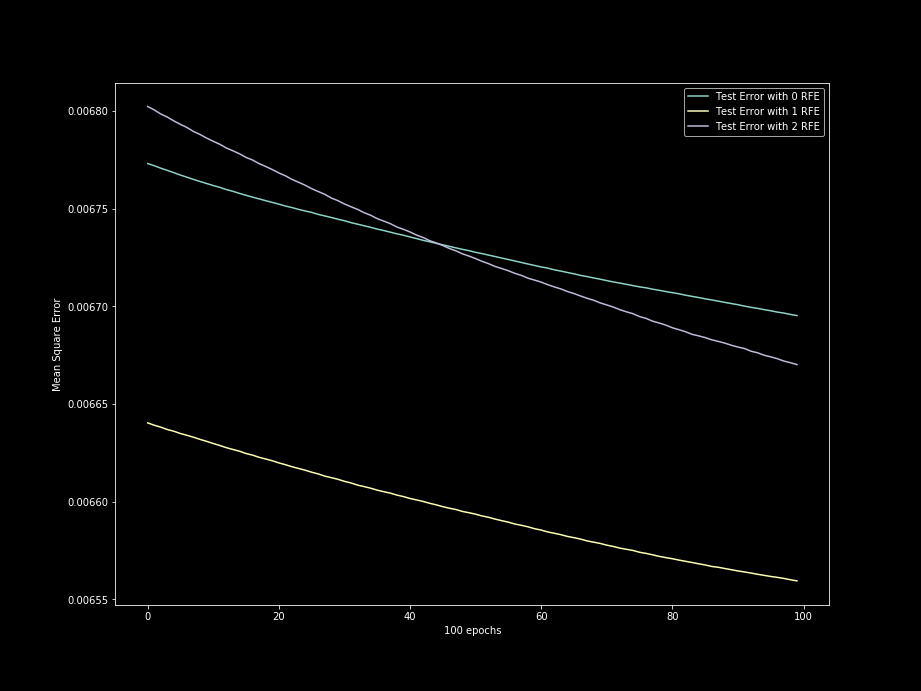
\includegraphics[width=0.8\linewidth]{assets/plots2/part3_8.png}
        \caption{Plot of accuracy predictions for different number of features removed by RFE - last 100 epochs}
        \label{fig:rfe3_zoom}
    \end{subfigure}
\end{figure}

As seen from Figure \ref{fig:rfe3_zoom}, the removal of just one feature (University Ranking) is the best for improving the model performance. The next iteration of RFE which removed SOP actually reduced the performance of the model to a level similar to when no RFE is performed. As such, the removal of just 1 feature is optimal in this case. A more detailed discussion will be discussed in the conclusion.

\subsection{Question 4}
\label{2q4}
\begin{quote}
4. Design a four-layer neural network and a five-layer neural network, with the hidden layers having 50 neurons each. Use a learning rate of $10^{-3}$ for all layers and optimal feature set selected in part (3). Introduce dropouts (with a keep probability of 0.8) to the layers and report the accuracies. Compare the performances of all the networks (with and without dropouts) with each other and with the 3-layer network.
\end{quote}
\begin{figure}[H]
    \begin{subfigure}{1\textwidth}
        \centering
        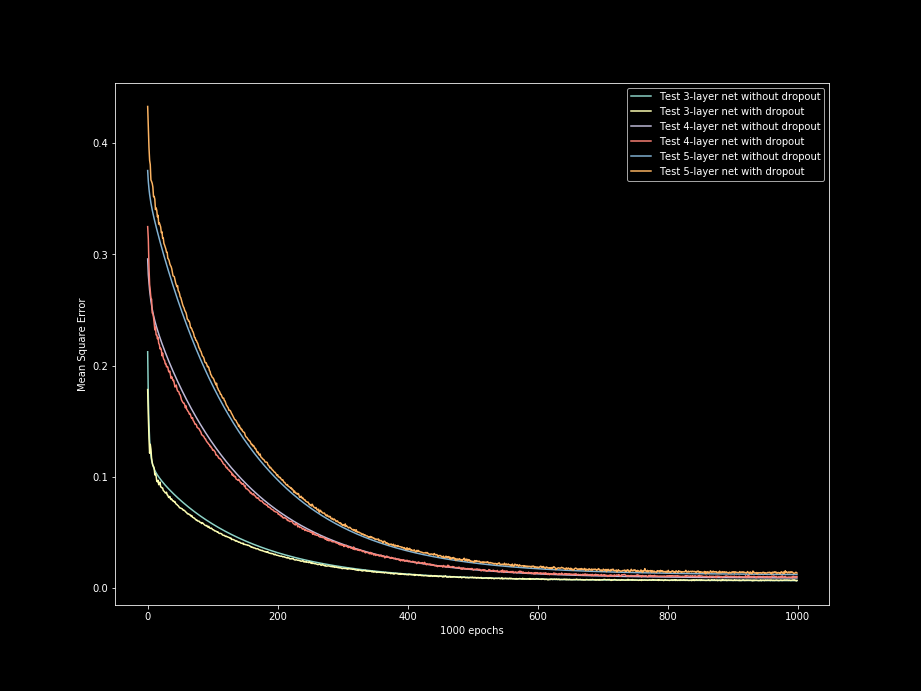
\includegraphics[width=0.8\linewidth]{assets/plots2/part4_1.png}
        \caption{Test errors for different network layers with and without dropout}
        \label{fig:2_4_1}
    \end{subfigure}
\end{figure}
\begin{figure}[H]
    \ContinuedFloat
    \begin{subfigure}{1\textwidth}
        \centering
        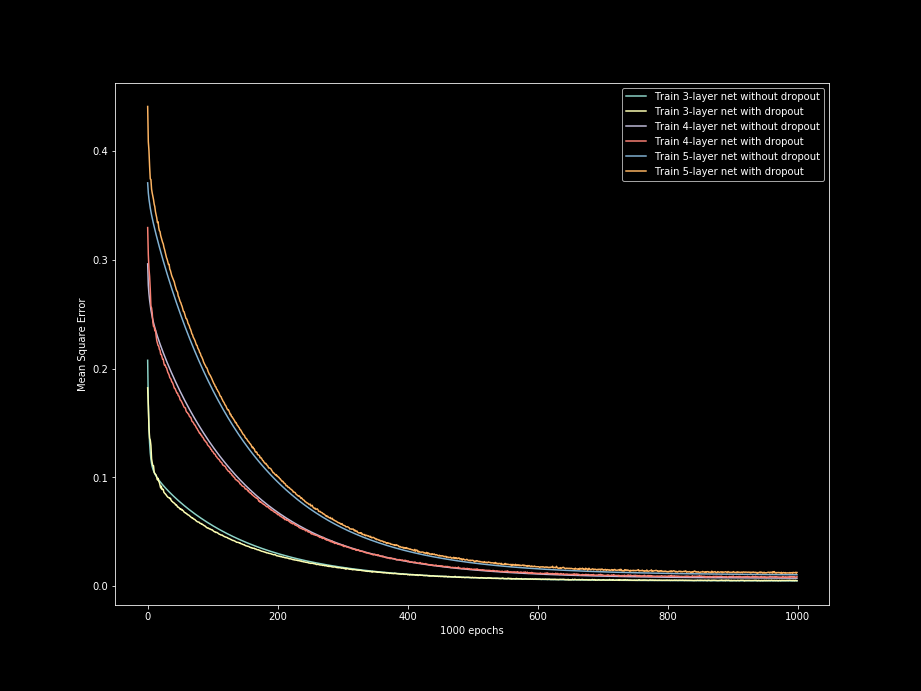
\includegraphics[width=0.8\linewidth]{assets/plots2/part4_2.png}
        \caption{Train errors for different network layers with and without dropout}
        \label{fig:2_4_2}
    \end{subfigure}
    \caption{Mean Square Errors for different network layers with and without dropout}
    \label{fig:2_4_3}
\end{figure}

From the results given in Figure \ref{fig:2_4_3}, for both \ref{fig:2_4_1} and \ref{fig:2_4_2}, we can see that the 3-layered network without dropout yields the least mean square error and it converges the fastest and yields the lowest mean square error, which means the best performance. Also, it has the least complexity by having only 3-layers, which reduces the tendency to overfit. For this dataset, a general trend can also be observed that as the number of layers increases, the mean square error and epoch to converge increases. The dropout reduces overfitting and thus improving the accuracy of the network itself, hence lower mean square error, better performance. Also generally, the introduction of dropouts will increase the performance of models in this regression dataset.
